\documentclass{ctexart}

\usepackage{graphicx}
\usepackage[hmargin=1.1in,vmargin=1in]{geometry}

\newcommand{\theauthor}{Sparky\_14145}

\input{personal_info/info.tex}

\title{计算机图形 作业二}
\author{\theauthor}

\begin{document}
    \maketitle

    \section{函数流程}

    \subsection{insideTriangle}

    如果一个点在三角形的内部,那么按照某一方向环绕三角形,则这个点会在任一条边的同一侧(具体哪一侧
    取决于环绕方向),即这个点 $P$ 到三角形的顶点 $V_1, V_2, V_3$ 的向量与这些边按照顺序所形成
    向量的外积($\overrightarrow{PV_1}\times\overrightarrow{V_1V_2}$, 
    $\overrightarrow{PV_2}\times\overrightarrow{V_2V_3}$,
    $\overrightarrow{PV_3}\times\overrightarrow{V_3V_1}$)方向(符号)相同。否则说明点不
    在三角形内(情况较多,省略讨论过程)。

    据此,直接计算 $\overrightarrow{PV_1}\times\overbrace{V_1V_2}$ 的符号,将另外两组外积
    的符号与之比较即可得出结果(相同说明点在三角形内,否则可能在外面或边上)。

    \subsection{rasterize\_triangle}

    找到三角形的顶点中 $x, y$ 分别的最大值和最小值,以这些最大最小值建立矩形,得到的便是一个粗略的
    ``bounding box''。然后轮询这个 box 中的所有像素点,检查它们是否位于三角形内,如果是则插值求
    出它的 $z$ 坐标,然后尝试更新 depth buffer。

    \section{运行结果}

    \begin{center}
        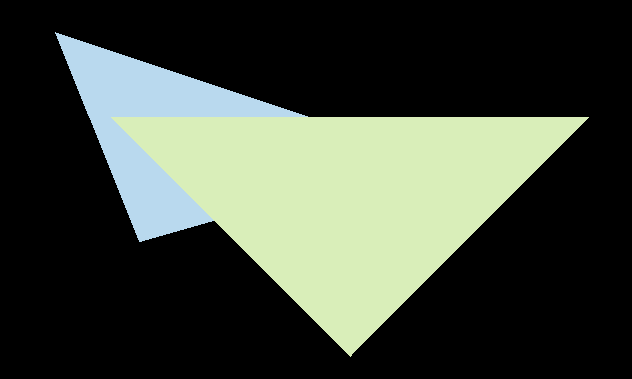
\includegraphics[width=0.6\textwidth]{pics/result.png}
    \end{center}
\end{document}